\documentclass[UTF8,12pt]{article}
\usepackage{ctex}
\usepackage{indentfirst}
\usepackage{color}
\usepackage{xcolor}
\usepackage{hyperref}
\usepackage{graphicx}
\usepackage{subfigure}
\usepackage{pdfpages}
\usepackage{listings}
\hypersetup{
    hidelinks,
	colorlinks=true,
	allcolors=black,
	pdfstartview=Fit,
	breaklinks=true
}

\definecolor{dkgreen}{rgb}{0,0.6,0}
\definecolor{gray}{rgb}{0.5,0.5,0.5}
\definecolor{mauve}{rgb}{0.58,0,0.82}

\lstset{ %
  language=Octave,                % the language of the code
  basicstyle=\footnotesize,           % the size of the fonts that are used for the code
  numbers=left,                   % where to put the line-numbers
  numberstyle=\tiny\color{gray},  % the style that is used for the line-numbers
  stepnumber=2,                   % the step between two line-numbers. If it's 1, each line 
                                  % will be numbered
  numbersep=5pt,                  % how far the line-numbers are from the code
  backgroundcolor=\color{white},      % choose the background color. You must add \usepackage{color}
  showspaces=false,               % show spaces adding particular underscores
  showstringspaces=false,         % underline spaces within strings
  showtabs=false,                 % show tabs within strings adding particular underscores
  frame=single,                   % adds a frame around the code
  rulecolor=\color{black},        % if not set, the frame-color may be changed on line-breaks within not-black text (e.g. commens (green here))
  tabsize=2,                      % sets default tabsize to 2 spaces
  captionpos=b,                   % sets the caption-position to bottom
  breaklines=true,                % sets automatic line breaking
  breakatwhitespace=false,        % sets if automatic breaks should only happen at whitespace
  title=\lstname,                   % show the filename of files included with \lstinputlisting;
                                  % also try caption instead of title
  keywordstyle=\color{blue},          % keyword style
  commentstyle=\color{dkgreen},       % comment style
  stringstyle=\color{mauve},         % string literal style
  escapeinside={\%*}{*)},            % if you want to add LaTeX within your code
  morekeywords={*,...}               % if you want to add more keywords to the set
}


\setlength{\parindent}{2em}

\begin{document}

\begin{titlepage}
    \includepdf[pages={1}]{cover.pdf}
\end{titlepage}

\begin{center}
    \tableofcontents
\end{center}
\newpage

\section{概要设计}
\subsection{实验目的与要求}
计算机体系结构是计算机专业学生的一门专业课程,本课程是计算机专业一门重要的专业课,着重讲述计算机系统的软、硬件界面。
对于学生从事计算机系统的研制、使用和维护有重要意义。本课程概念多、内容涉及面广、系统性强。
通过本课程的学习,学生应能从软件、硬件功能分配的角度去了解、分析和研究计算机系统,建立起对计算机系统的全面认识,树立全面地、发展地看问题的观点,从而加深对各种类型体系结构的了解,牢固地树立起整机系统的概念。

本课程的学习应注重理论与实践相结合,因此实验教学是教学环节中必不可少的重要内容。通过实验教学的学习,使学生熟练掌握有关计算机体系结构的基本概念、基本原理和基本思想,掌握对计算机体系结构和组成进行分析和计算的方法。

实验部分包括四个实验,包括有完整的源程序例题,介绍了一些设计数据结构题目所需的的知识和技巧。在实验题中,既有简单容易的验证题,即验证已经给出的源程序,或者扩充已经给出的源程序,也有需独立思考设计的综合实验题。

\subsection{开发环境}
\begin{itemize}
    \item 操作系统:Windows 11
    \item 开发环境:Dev-C++ 5.11
    \item 编程语言:C++
\end{itemize}

\newpage

\section{实验一}
\subsection{实验题目}
对指令操作码进行霍夫曼编码

\subsection{实验目的}
\begin{itemize}
    \item 了解和掌握指令编码的基本要求和基本原理
\end{itemize}

\subsection{实验内容}
使用编程工具编写一个程序,对一组指令进行霍夫曼编码,并输出最后的编码结果以及对指令码的长度进行评价,与扩展操作码和等长编码进行比较。

例如,有一组指令的操作码共分七类,它们出现概率如下表所示:
\begin{table}[htbp]
\centering
\begin{tabular}{c|c|c|c|c|c|c|c}
\hline
指令   & P1   & P2  & P3   & P4   & P5   & P6   & P7   \\ \hline
出现概率 & 0.45 & 0.30 & 0.15 & 0.05 & 0.03 & 0.01 & 0.01 \\ \hline
\end{tabular}
\end{table}

对此组指令进行Huffman编码如下图所示:
\begin{figure}[htbp]
    \centering
    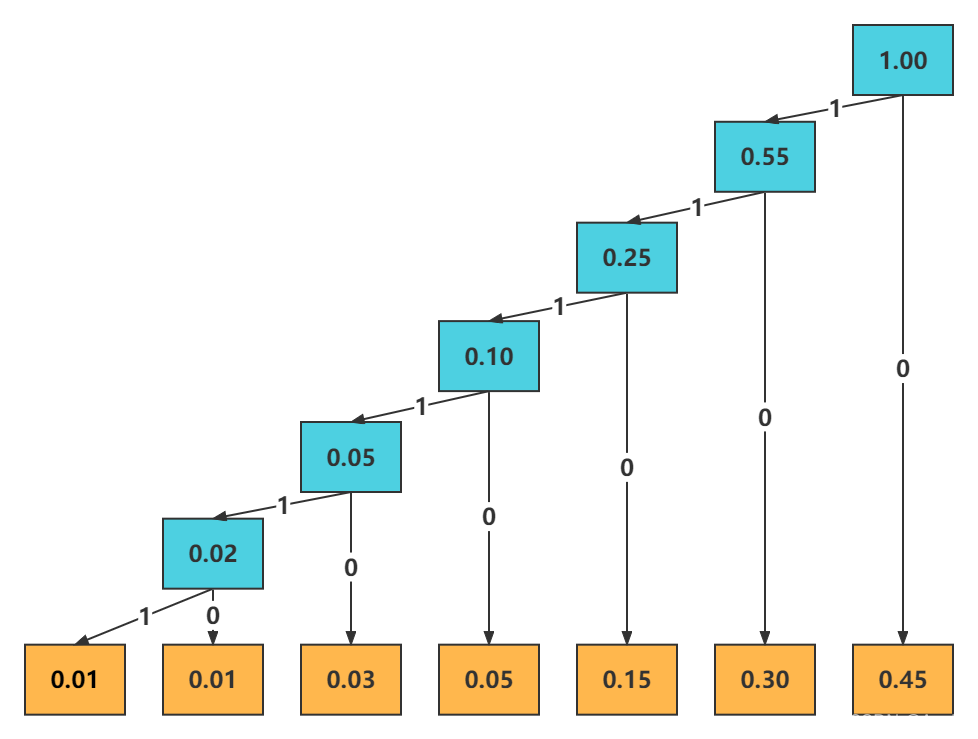
\includegraphics[width=0.5\textwidth]{imgs/1.png}
    \caption{Huffman编码}
\end{figure}

最后得到的Huffman编码如下表所示:

\begin{table}[htbp]
    \centering
    \begin{tabular}{cccccccc}
    \hline
    \textbf{指令}        & \textbf{P1} & \textbf{P2} & \textbf{P3}  & \textbf{P4}   & \textbf{P5}    & \textbf{P6}     & \textbf{P7}     \\ \hline
    出现概率               & 0.45        & 0.3         & 0.15         & 0.05          & 0.03           & 0.01            & 0.01            \\
    \textbf{Huffman编码} & \textbf{0}  & \textbf{10} & \textbf{110} & \textbf{1110} & \textbf{11110} & \textbf{111110} & \textbf{111111} \\
    编码长度               & 1           & 2           & 3            & 4             & 5              & 6               & 6               \\ \hline
    \end{tabular}
\end{table}

通过上面表格可以计算得到最毒按的编码长度:
$$
H=0.45\times1+0.30\times2+0.15\times3+0.05\times4+0.03\times5+0.01\times6+0.01\times6=1.97
$$

要对指令的操作码进行Huffman编码,只要根据指令的各类操作码的出现概率构造Huffman树再进行Huffman编码。此过程的难点构造Huffman树,进行Huffman编码只要对你所生成的Huffman树进行中序遍历即可完成编码工作

\subsection{实验过程}
观察上图1,不难看出构造Huffman树所要做的工作:

\begin{enumerate}
    \item 先对各指令操作码的出现概率进行排序,构造一个有序链表。
    \item 再取出两个最小的概率节点相加,生成一个生的节点加入到链表中,同时从两表中删除此两个节点。
    \item 在对链表进行排序,链表是否只有一个节点,是则Huffman树构造完毕,否则继续做2的操作。
\end{enumerate}

\newpage

为此设计一个工作链表(链表的元素时类,此类的功能相当结构。)、HHuffman树节点、Huffman编码表节点。具体如下:


\begin{lstlisting}[frame=shadowbox] 
    // huffman树节点类
    class huff_p {
    public:
        huff_p* r_child;  // 大概率的节点
        huff_p* l_child;  // 小概率的节点
        char op_mask[3];  // 指令标号
        float p;          // 指令使用概率
    };
    
    // 最小概率节点链表节点类
    class f_min_p {
    public:
        f_min_p* next;
        char op_mask[3];   // 指令标号
        float p;           // 指令使用概率
        huff_p* huf_p;      // 对应的huffman树节点
    };
    
    // huffman编码节点类
    class huff_code {
    public:
        huff_code* next;
        float p;
        char op_mask[3];
        char code[N];      // huffman 编码
    };
    
    // 输入指令集子模块
    f_min_p* input_instruct_set();
    
    // 构造huffman树
    huff_p* creat_huffman_tree(f_min_p* head);
    
    // 在最小概率节点链表中找到概率最小的节点
    f_min_p* fin_min(f_min_p* h);
    
    // 从最小概率节点链表中删除指定节点
    f_min_p* del_min(f_min_p* h, f_min_p* p);
    
    // 将新节点按概率插入到最小概率节点链表中合适的位置
    void insert_n(f_min_p* h, f_min_p* p);
    
    // 根据最小概率节点创建huffman树节点
    huff_p* creat_huffp(f_min_p* p);
    
    // 递归生成huffman编码
    void r_find(huff_p* p1, char code[], int i, huff_code* h);
    
    // 生成huffman编码
    void creat_huffman_code(huff_p* h1, huff_code* h);
    
    // 输出huffman编码
    void output_huffman(huff_code* head);
    
    // 计算指令用huffman编码的平均编码字长
    void cal_sort_length(huff_code* head);
    
    // 打印huffman树
    void print(huff_p* h1);
\end{lstlisting}

以上是实验指导书中给出的数据结构,有一些错误和不完善之处,我进行了修改和完善

下面针对重要函数申明展开说明:

\subsubsection{构造huffman树}
\begin{lstlisting}[frame=shadowbox] 
    huff_p* creat_huffman_tree(f_min_p* h) {
        f_min_p* h1, *min1, *min2, *comb;
        huff_p* head, *rd, *ld, *parent;
        h1 = h;
    
        min1 = fin_min(h1);
        ld = creat_huffp(min1);
        h1 = del_min(h1, min1);
    
        if (h1->next) {
            min2 = fin_min(h1);
        }
        else {
            min2 = h1;
        }
    
        rd = creat_huffp(min2);
        comb = new f_min_p;
        comb->next = NULL;
        comb->p = rd->p + ld->p;
        comb->op_mask[0] = '\0';
        comb->op_mask[1] = '\0';
    
        parent = creat_huffp(comb);
    
        insert_n(h1, comb);
        if (h1->next != NULL) {
            h1 = del_min(h1, min2);
        }
    
        parent->l_child = ld;
        parent->r_child = rd;
    
        comb->huf_p = parent;
    
        head = parent;
        while (h1->next != NULL) {
            min1 = fin_min(h1);
            if (min1->huf_p == NULL) {
                ld = creat_huffp(min1);
            }
            else {
                ld = min1->huf_p;
            }
            h1 = del_min(h1, min1);
    
            if (h1->next) {
                min2 = fin_min(h1);
            }
            else {
                min2 = h1;
            }
            if (min2->huf_p == NULL) {
                rd = creat_huffp(min2);
            }
            else {
                rd = min2->huf_p;
            }
            comb = new f_min_p;
            comb->next = NULL;
            comb->p = rd->p + ld->p;
            comb->op_mask[0] = '\0';
            comb->op_mask[1] = '\0';
            parent = creat_huffp(comb);
            if (h1 != NULL) {
                insert_n(h1, comb);
            }
    
            if (h1->next != NULL) {
                h1 = del_min(h1, min2);
            }
            if (h1->next == NULL && ld->p < rd->p) {
                huff_p* tmp = ld;
                ld = rd;
                rd = tmp;
            }
            parent->l_child = ld;
            parent->r_child = rd;
            comb->huf_p = parent;
            head = parent;
    
            if (h1->next == NULL) {
                break;
            }
        }
        delete comb;
        return head;
    }
\end{lstlisting}

creat\_huffman\_tree()函数用于构造Huffman树,返回Huffman树的根节点。

实现流程如下:
\begin{enumerate}
    \item 通过fin\_min函数找到堆中的最小频率节点,并使用creat\_huffp函数创建一个哈夫曼节点,将其作为左子树。
    \item 从堆中删除找到的最小频率节点。
    \item 判断堆中是否还有节点,如果有,则继续找到第二个最小频率节点,并创建右子树,然后将两个最小节点的频率相加,构建一个新的频率最小堆节点comb,并将其作为父节点。
    \item 将左右子树链接到父节点。
    \item 将父节点插入堆中,并从堆中删除之前找到的最小频率节点。
    \item 将新的父节点作为根节点,循环以上步骤,直到堆中只剩一个节点,即哈夫曼树的根节点。
\end{enumerate}

\subsubsection{在最小概率节点链表中找到概率最小的节点}
\begin{lstlisting}[frame=shadowbox] 
    f_min_p* fin_min(f_min_p* h) {
        f_min_p* h1, *p1;
        h1 = h;
        p1 = h1;
        float min = h1->p;
        h1 = h1->next;
        while (h1) {
            if (min > (h1->p)) {
                min = h1->p;
                p1 = h1;
            }
            h1 = h1->next;
        }
        return p1;
    }
\end{lstlisting}

fin\_min()函数用于在最小概率节点链表中找到概率最小的节点,返回该节点的指针。这一函数通过遍历整个链表,找到概率最小的节点。

\subsubsection{从最小概率节点链表中删除指定节点}
\begin{lstlisting}[frame=shadowbox] 
    f_min_p* del_min(f_min_p* h, f_min_p* p) {
        f_min_p* p1, *p2;
        p1 = h;
        p2 = h;
        if (h == p) {
            h = h->next;
            delete p;
        }
        else {
            while (p1->next != NULL) {
                p1 = p1->next;
                if (p1 == p) {
                    p2->next = p1->next;
                    delete p;
                    break;
                }
                p2 = p1;
            }
        }
        return h;
    }
\end{lstlisting}

del\_min()函数用于从最小概率节点链表中删除指定节点,返回删除后的链表。这一函数通过遍历整个链表,找到指定节点,然后删除该节点。

\subsubsection{将新节点按概率插入到最小概率节点链表中合适的位置}
\begin{lstlisting}[frame=shadowbox] 
    void insert_n(f_min_p* h, f_min_p* p1) {
        p1->next = h->next;
        h->next = p1;
    }
\end{lstlisting}

insert\_n()函数用于将新节点按概率插入到最小概率节点链表中合适的位置。这一函数是将新节点插入到链表的第二个位置,第一个位置是头节点。

\subsubsection{根据最小概率节点创建huffman树节点}
\begin{lstlisting}[frame=shadowbox] 
    huff_p* creat_huffp(f_min_p* d) {
        huff_p* p1;
        p1 = new huff_p;
        p1->l_child = NULL;
        p1->r_child = NULL;
        p1->p = d->p;
        p1->op_mask[0] = d->op_mask[0];
        p1->op_mask[1] = d->op_mask[1];
        return p1;
    }
\end{lstlisting}

creat\_huffp()函数用于根据最小概率节点创建huffman树节点,返回创建的节点。这一函数是将最小概率节点转换为哈夫曼树节点。

\subsubsection{递归生成huffman编码}
\begin{lstlisting}[frame=shadowbox] 
    void r_find(huff_p* p1, char code[], int i, huff_code* h) {
        if (p1->l_child) {
            code[i] = '1';
            r_find(p1->l_child, code, i + 1, h);
        }
        if (p1->op_mask[0] != '\0') {
            huff_code* p2 = new huff_code;
            p2->op_mask[0] = p1->op_mask[0];
            p2->op_mask[1] = p1->op_mask[1];
            p1->op_mask[2] = '\0';
            p2->p = p1->p;
            int j = 0;
            for (; j < i; j++) {
                p2->code[j] = code[j];
            }
            p2->code[j] = '\0';
            p2->next = h->next;
            h->next = p2;
        }
        if (p1->r_child) {
            code[i] = '0';
            r_find(p1->r_child, code, i + 1, h);
        }
        delete p1;
    }
\end{lstlisting}

r\_find()函数用于递归生成huffman编码,返回生成的编码。这一函数是通过递归遍历哈夫曼树,将遍历到的节点的编码保存到编码表中。

\subsubsection{生成huffman编码}
\begin{lstlisting}[frame=shadowbox] 
    void creat_huffman_code(huff_p* h1, huff_code* h) {
        int i = 0;
        char code[N] = { '\0' };
        r_find(h1, code, i, h);
    }
\end{lstlisting}

creat\_huffman\_code()函数用于生成huffman编码,返回生成的编码。这一函数是通过调用r\_find()函数,将遍历到的节点的编码保存到编码表中。

\newpage

\subsection{实验结果}
\begin{figure}[htbp]
    \centering
    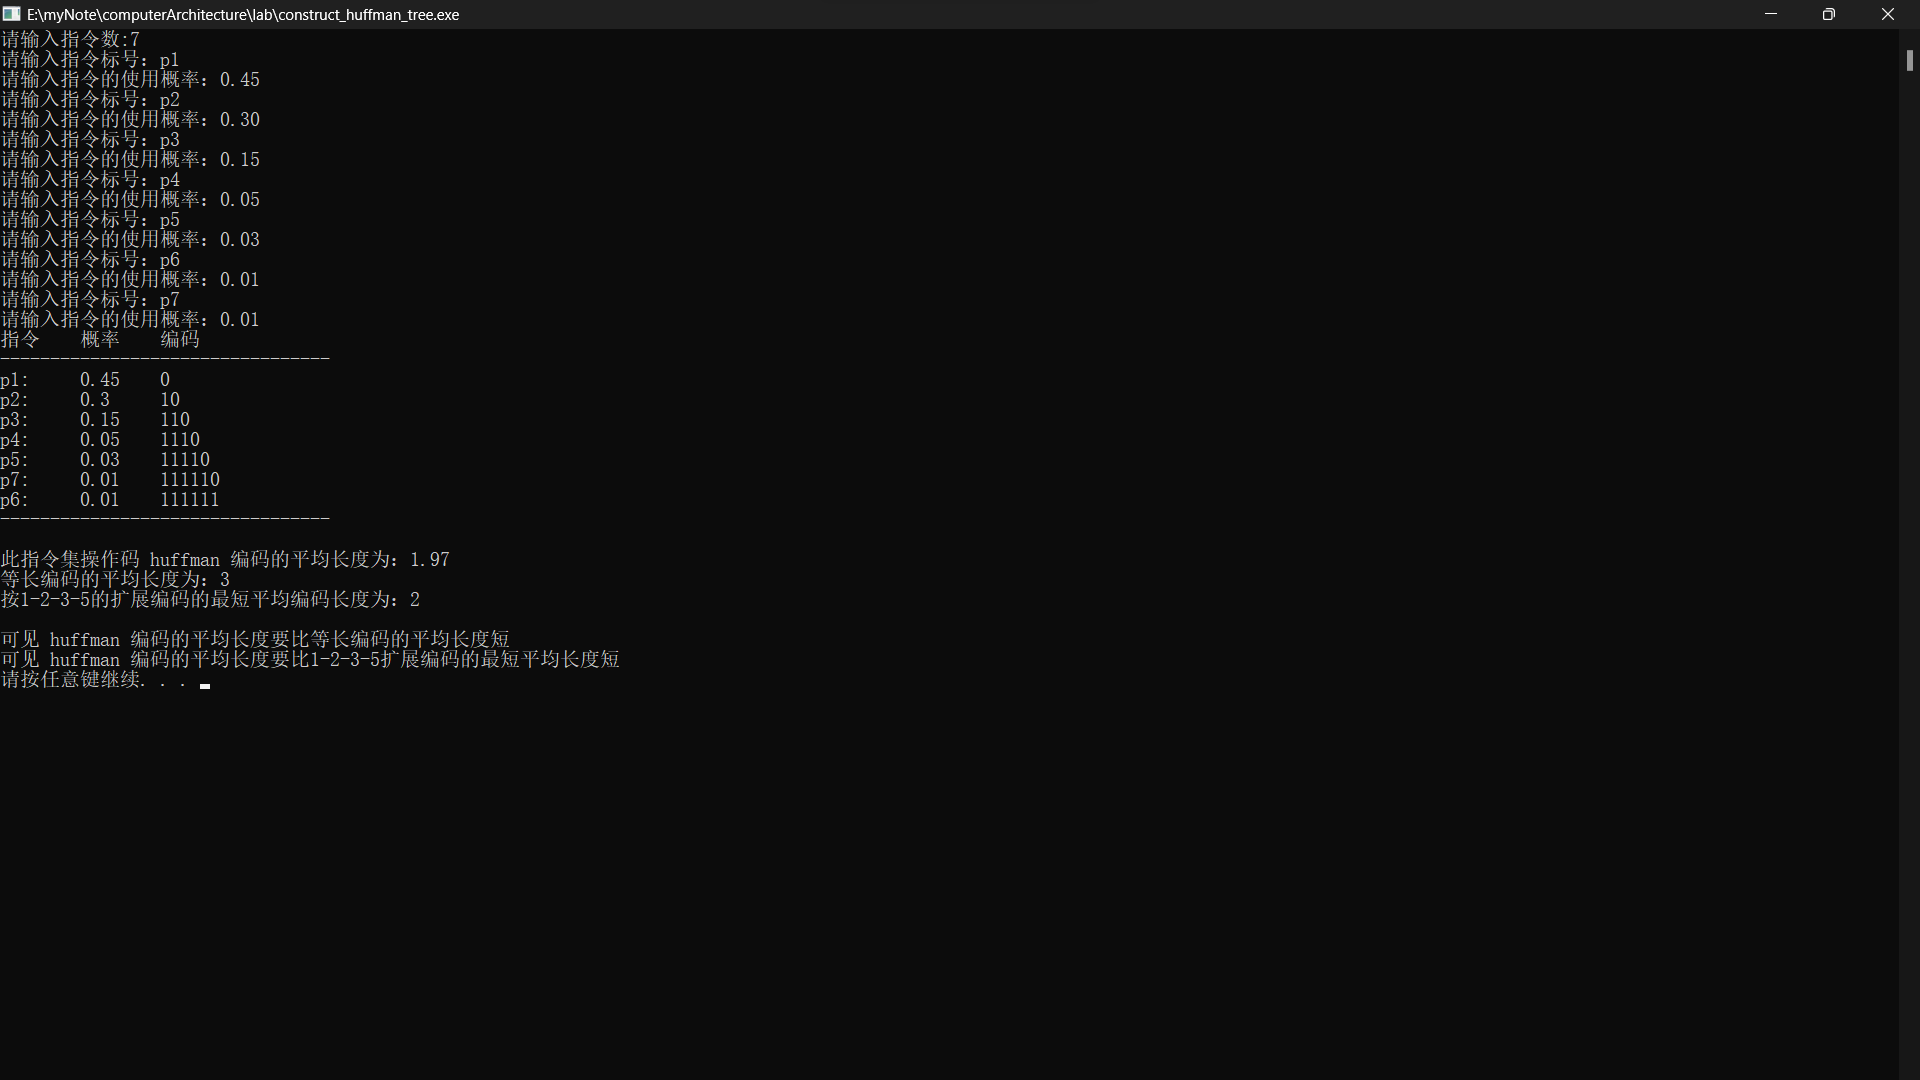
\includegraphics[width=1.0\textwidth]{imgs/2.png}
    \caption{实验一实验结果}
\end{figure}

\newpage

\section{实验二}
\subsection{实验题目}
使用LRU方法更新Cache

\subsection{实验目的}
\begin{itemize}
    \item 了解和掌握寄存器分配和内存分配的有关技术
\end{itemize}

\subsection{实验内容}
结合数据结构的相关知识,使用LRU的策略,对一组访问序列进行内部的Cache更新

LRU置换算法是选择最近最久未使用的页面予以置换。该算法赋予每个页面一个访问字段,用来记录一个页面自上次被访问以来经历的时间T,当须淘汰一个页面时,选择现有页面中T值最大的,即最近最久没有访问的页面。这是一个比较合理的置换算法。

举例说明此问题,例如:

有一个Cache采用组相连映象方式。每组有四块,为了实现LRU置换算法,在快表中为每块设置一个2位计数器。我们假设访问序列为“1,1,2,4,3,5
,2,1,6,7,1,3”。在访问Cache的过程中,块的装入,置换及命中时,具体情况如下表所示:

\begin{table}[htbp]
    \begin{tabular}{ccccccccccccc}
    \hline
            & 1  & 1  & 2  & 4  & 3  & 5  & 2  & 1  & 6  & 7  & 1  & 3  \\ \hline
    Cache块0 & 1  & 1  & 1  & 1  & 1  & 5  & 5  & 5  & 5  & 7  & 7  & 7  \\
    Cache块1 &    &    & 2  & 2  & 2  & 2  & 2  & 2  & 2  & 2  & 2  & 3  \\
    Cache块2 &    &    &    & 4  & 4  & 4  & 4  & 1  & 1  & 1  & 1  & 1  \\
    Cache块3 &    &    &    &    & 3  & 3  & 3  & 3  & 6  & 6  & 6  & 6  \\
            & 装入 & 命中 & 装入 & 装入 & 装入 & 置换 & 命中 & 置换 & 置换 & 置换 & 命中 & 置换 \\ \hline
    \end{tabular}
\end{table}

\subsection{实验过程}
在这个模拟实验中,首先需要建立模拟的Cache类具体实现如下:

\begin{lstlisting}[frame=shadowbox] 
    class Cache {
public:
    bool state = false;  // Cache块的状态,false表示空闲,true表示占用
    int value = -1;      // Cache块存储的数值
    int count = 0;       // Cache块的未使用时间计数
};
\end{lstlisting}

最重要的是实现LRU算法,实现如下:

\begin{lstlisting}[frame=shadowbox] 
    void up_cache() {
        int i = 0;
        while (i < N) {
            int j = 0;
               // 是否已满 
               cout << endl;
               cout << "--------------p" << walk_sort[i] << "到达--------------" << endl;
               cout << endl;
            while (j < M) {
                if((cache[j].state == false) && (walk_sort[i] != cache[j].value)) {
                    cout << "cache有空闲块,不考虑是否要置换..." << endl;
                    cout << walk_sort[i] << "被装入cache...." << endl;
                    //cache[j].value = walk_sort[i++]; 
                    cache[j].value = walk_sort[i]; 
                    cache[j].state = true;
                    cache[j].count = 0;
                    int kk = 0;
                    
                    for (int x = 0; x < M; x++) {
                        cout << "cache块" << x << ": " << cache[x].value << endl;
                    }
                    cout << endl;
                    
                    // 更新其它cache块没使用时间
                    while (kk < M) {
                        if (kk != j && cache[kk].value != -1) {
                            cache[kk].count++;
                        }
                        kk++;
                    }
                    break; 
                }
                
                if (cache[j].value == walk_sort[i]) {
                    cout << endl;
                    cout << walk_sort[i] << "命中!!!" << endl;
                    
                    for (int x = 0; x < M; x++) {
                        cout << "cache块" << x << ": " << cache[x].value << endl;
                    }
                    cout << endl;
                    //i++; 
                    int kk = 0;
                    cache[j].count=0;
                    //更新其它cache块没使用时间
                    while (kk < M) {
                        if (kk != j && cache[kk].value != -1) {
                            cache[kk].count++;
                        }
                        kk++;
                    }
                    break;
                }
                j++;
            }
    
            //cache已满 
            if (j == M) {
                cout << "cache已经满了,考虑是否置换..." << endl;
                cout << endl;
                int k = 0;
    
                while (k < M) {
                    if (cache[k].value == walk_sort[i]) {
                        cout << endl;
                        cout << walk_sort[i] << "命中!!!" << endl;
      
                        for (int x = 0; x < M; x++) {
                            cout << "cache块" << x << ": " << cache[x].value << endl;
                        }
                        
                        //i++;
                        cache[k].count = 0;
                        int kk = 0;
                         
                        //更新其它cache块没使用时间
                        while (kk < M) {
                            if (kk != k){
                                cache[kk].count++;
                            }
                            kk++;
                        }
                        break;
                    }
                    k++;
                } 
                
                //考虑置换哪一块 
                if (k == M) {
                    int ii = 0;
                    int t = 0;//要替换的cache块号.
                    int max = cache[ii].count;
                    ii++; 
                    while (ii < M) {
                        if(cache[ii].count > max) {
                            max = cache[ii].count;
                            t = ii;
                        }
                        ii++;
                    }
                    //置换
                    cout<<cache[t].value<<"被"<<walk_sort[i]<<"在cache的"<<t<<"号块置换..."<<endl;
                    //cache[t].value=walk_sort[i++];
                    cache[t].value=walk_sort[i];
                    cache[t].count=0;
                    
                    for (int x = 0; x < M; x++) {
                        cout << "cache块" << x << ": " << cache[x].value << endl;
                    }
                    int kk = 0;                
                    //更新其它cache块没使用时间
                    while (kk < M) {
                        if (kk != t) {
                            cache[kk].count++;
                        }
                        kk++;
                    }
                }
            }
            i++;
        }
    }
\end{lstlisting}

具体实现流程如下:
\begin{enumerate}
    \item 外层循环通过遍历输入数组walk\_sort中的元素,逐个处理每个元素。
    \item 内层循环遍历缓存数组cache,查找是否有缓存块的值与当前输入元素相等。
    \item 如果找到相等的缓存块,输出命中信息,更新缓存块的未使用时间,并跳出内层循环。
    \item 如果没有找到相等的缓存块,检查是否有空闲缓存块,如果有,则将当前输入元素装入空闲缓存块,并更新相关信息。
    \item 如果缓存已满且没有找到相等的缓存块,则根据缓存块的未使用时间选择要替换的缓存块,选择未使用时间最长的缓存块进行替换并进行替换操作。
    \item 输出相关信息,更新缓存块的未使用时间。
    \item 继续处理下一个输入元素。
\end{enumerate}

\newpage

\subsection{实验结果}
\begin{figure}[htbp]
    \centering
    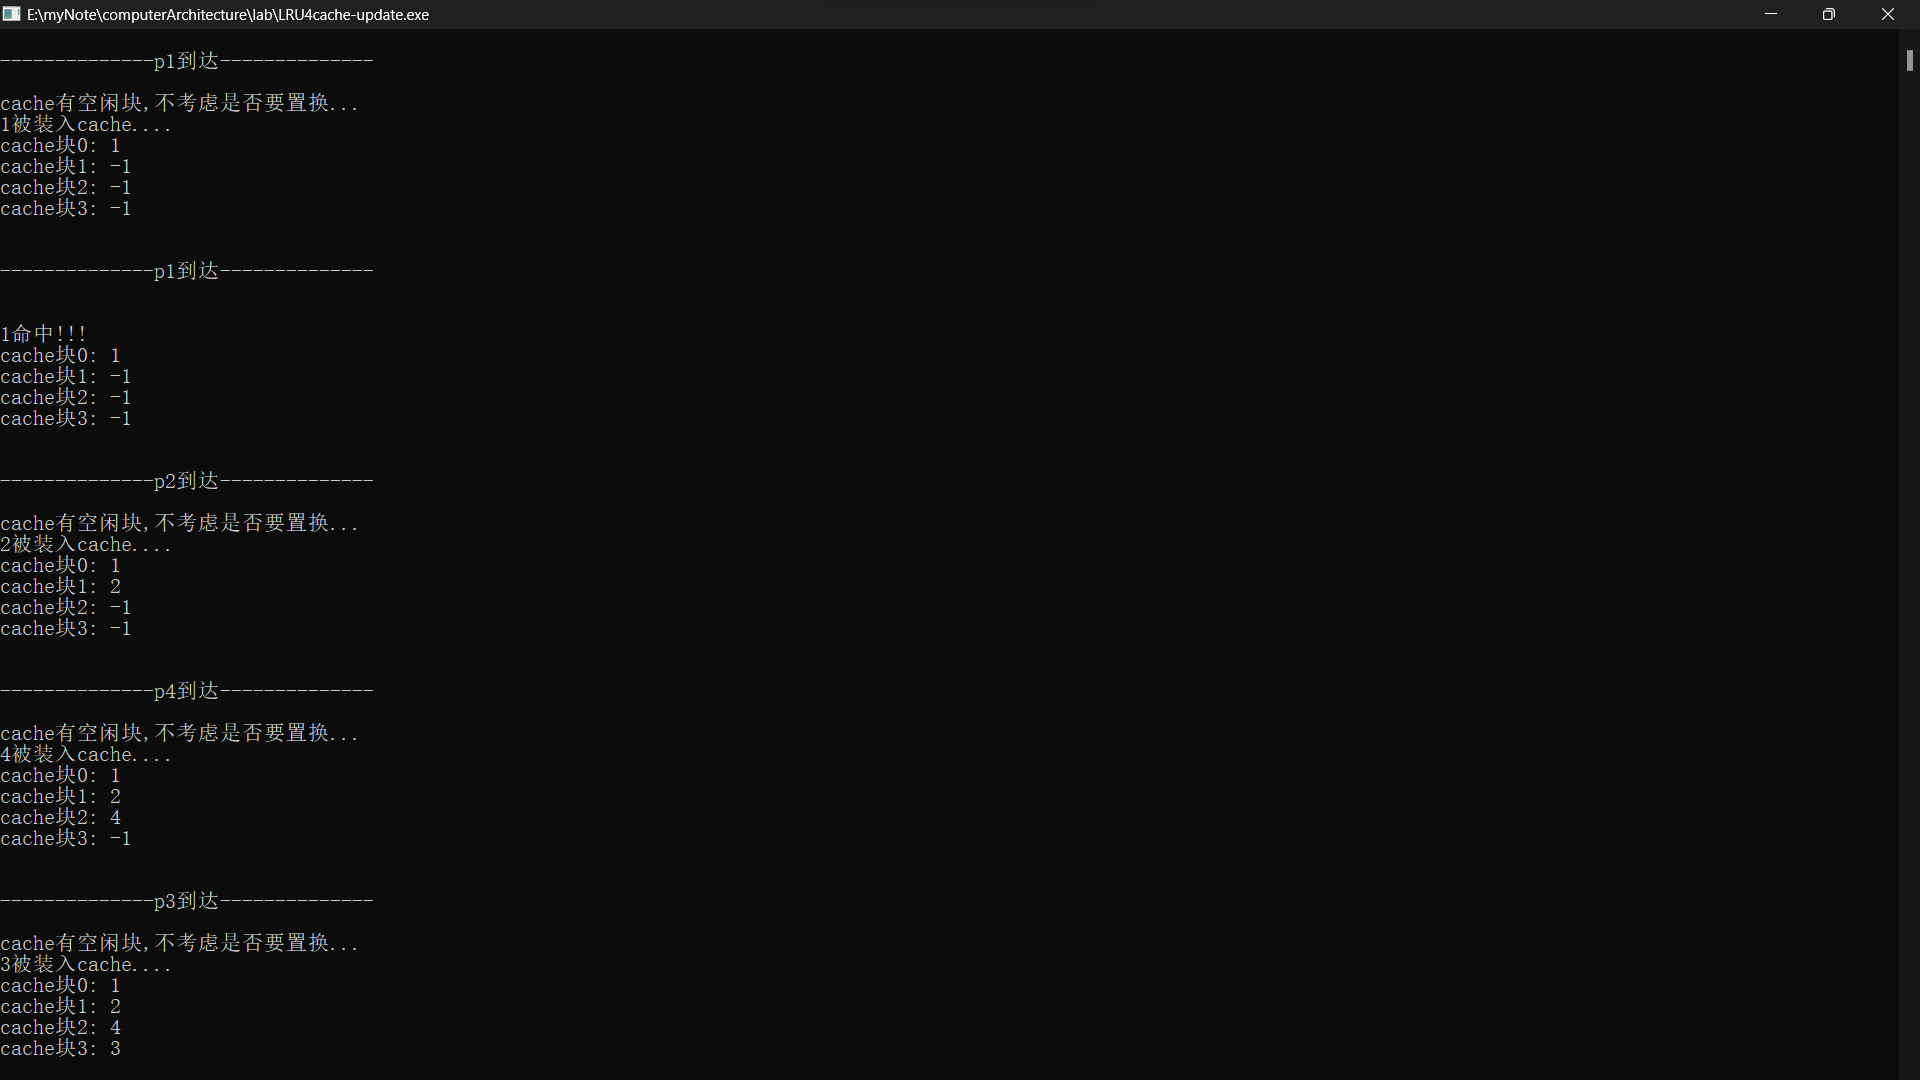
\includegraphics[width=0.7\textwidth]{imgs/3.png}
    \caption{实验二实验结果1}
\end{figure}

\begin{figure}[htbp]
    \centering
    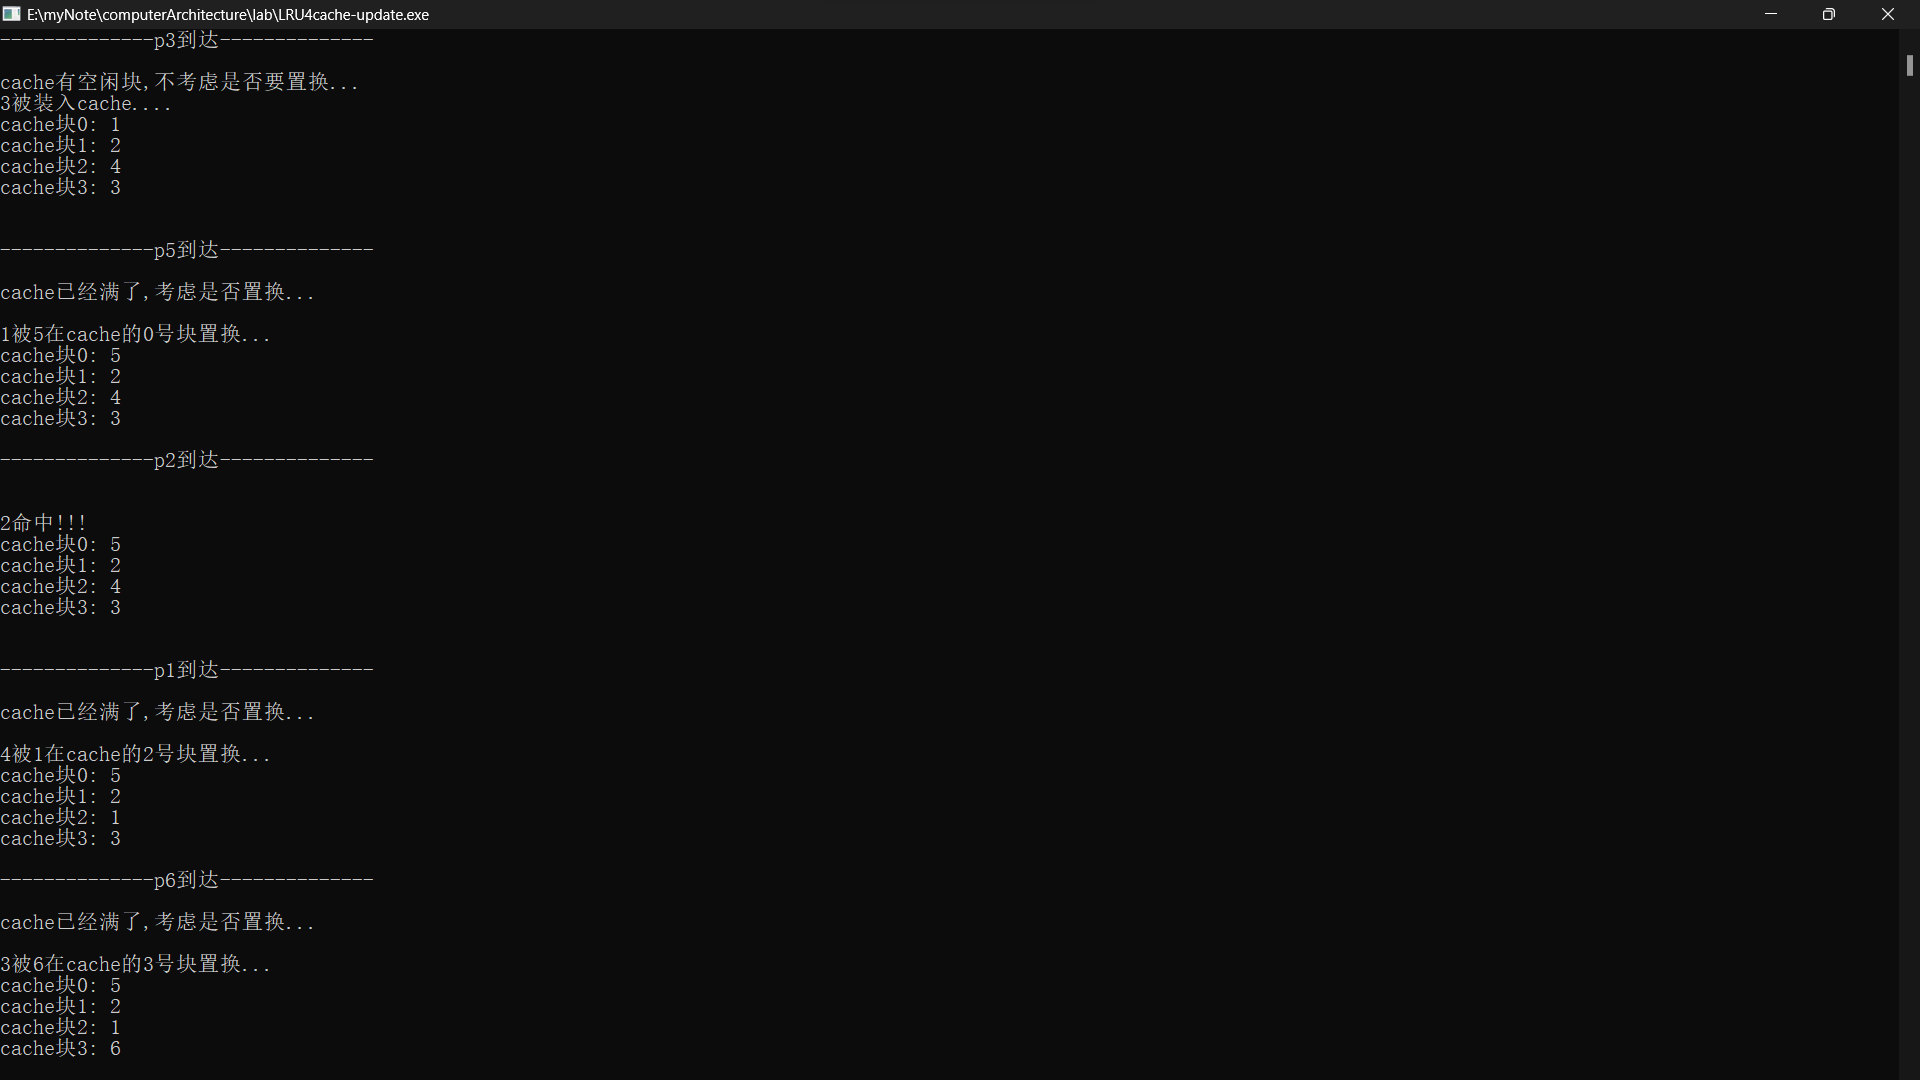
\includegraphics[width=0.7\textwidth]{imgs/4.png}
    \caption{实验二实验结果2}
\end{figure}

\begin{figure}[htbp]
    \centering
    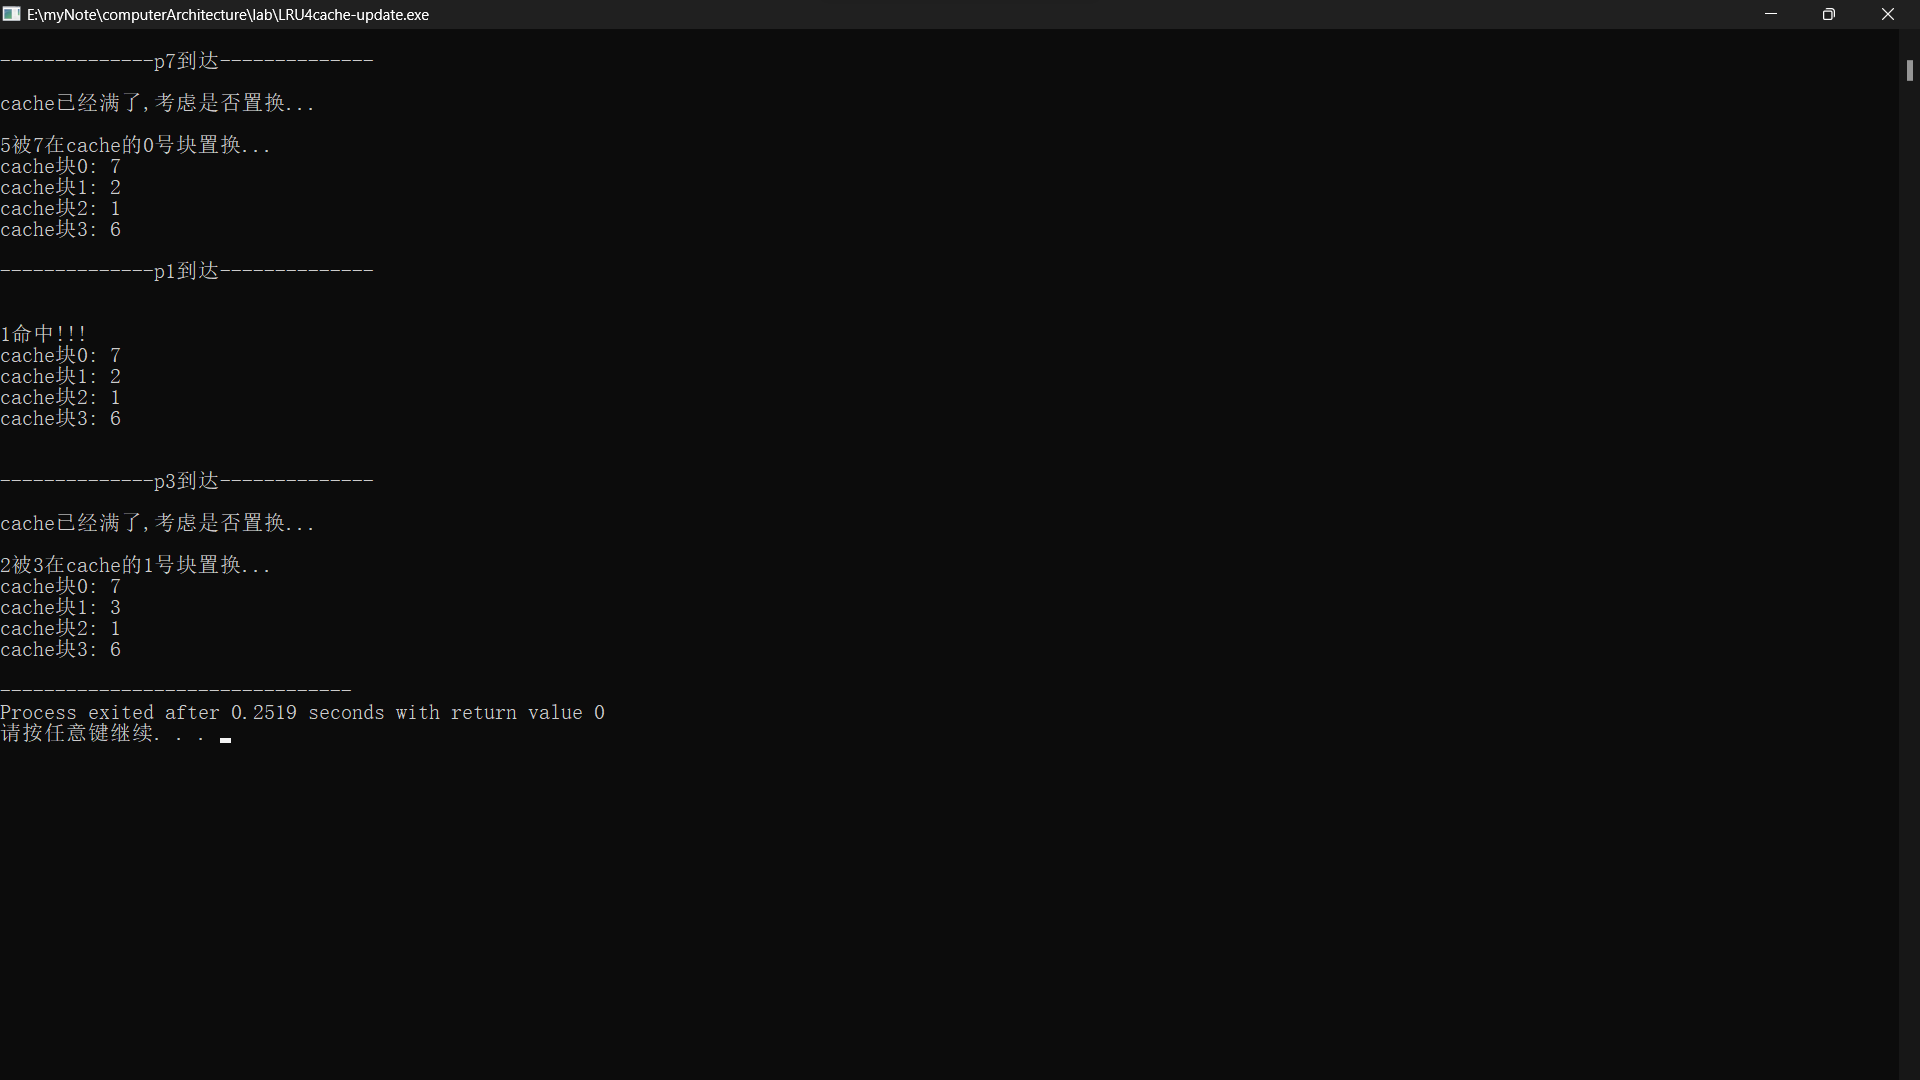
\includegraphics[width=0.8\textwidth]{imgs/5.png}
    \caption{实验二实验结果3}
\end{figure}

\newpage

\section{实验三}

\subsection{实验题目}
通道处理过程模拟

\subsection{实验目的}
通过模拟实现通道处理过程,掌握通道技术。

\subsection{实验内容}
结合数据结构的相关知识,编写通道处理过程模拟程序。

通道完成一次数据输入输出的过程需三步(如图所示):
\begin{enumerate}
    \item 在用户程序中使用访管指令进入管理程序,由CPU通过管理程序组织一个通道程序,并启动通道;
    \item 通道处理机执行通道程序,完成指定的数据输入输出工作;
    \item 通道程序结束后第二次调用管理程序对输入输出请求进行处理每完成一次输入输出工作,CPU只需要两次调用管理程序,大大减少了对用户程序的打扰。    
\end{enumerate}

\begin{figure}[htbp]
    \centering
    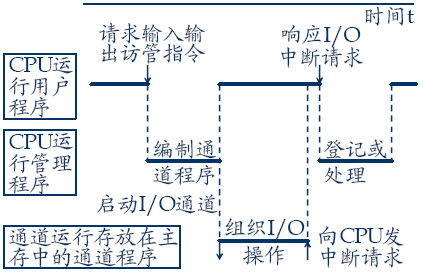
\includegraphics[width=0.8\textwidth]{imgs/6.png}
    \caption{通道处理过程}
\end{figure}

\subsection{实验过程}
通道处理过程的一些操作比较复杂,因此将其分为三个类Memory类、Device类和Ch\_mannager类来实现,分别对应内存、设备和通道管理程序。

\subsubsection{Memory类}
\begin{lstlisting}[frame=shadowbox] 
    class Memory {
        private:
            char* itsString;
            int itsLen;
        public:
            Memory();
            Memory(const char* content);
            ~Memory();
            void SetMcontent(const char* content);
            char* GetMcontent() const {
                return this->itsString;
            }
    };
\end{lstlisting}

Memory类用于模拟内存,其主要功能是存储数据。

\subsubsection{Device类}
\begin{lstlisting}[frame=shadowbox] 
    class Device {
        private:
            int Num;
            int RequireTime;
            int priority;
            char* Content;
            int itslen;
            int RequireState;// 0->r 1-> nr
            int itspos;
        public:
            Device();
            Device(int itsNum,int itsRequireTime);
            ~Device() {
                delete[] Content;
            }
            void SetNum(int itsNum);
            int GetNum() {
                return Num;
            }
            void SetRequireTime(int itsRequireTime);
            int GetRequireTime() {
                return RequireTime;
            }
            void Setpriority(int itspriority);
            int Getpriority() {
                return priority;
            }
            void SetContent(const char* itscontent);
            char* GetContent() const {
                return this->Content;
            }
            void SetRequireState(int state);
            int GetRequireState() {
                return RequireState;
            }
            void PrintDevice();
    // int operator++(){ return itspos++; };
            int Getpos() {
                return itspos;
            }
    };
\end{lstlisting}

Device类用于模拟设备,其主要功能是模拟请求中断的设备。

\subsubsection{Ch\_mannager类}
\begin{lstlisting}[frame=shadowbox]
    class Ch_mannager {
	public:
		Ch_mannager() {}
		~Ch_mannager() {}
		void run(int state);
		int sort(Device []);
		void memoryToDevice(Memory [],Device []);
    };
\end{lstlisting}

Ch\_mannager类用于模拟通道管理程序,其主要功能是模拟通道管理程序的运行,在这个类里面实现了管道管理的算法,就是memoryToDevice()函数。

传输方式为内存到设备,采用字节多路方式,设备分时复用通道的工作算法,具体实现如下:

\begin{lstlisting}[frame=shadowbox] 
void Ch_mannager::memoryToDevice(Memory m[],Device d[]) {
	int i;
	int maxDnum = 0;
	int flag = 0;
	static int time = 0;
	for(i = 0; i < 4; i++) {
		d[i].SetRequireState(1);
	}

	while(true) {
		cout << "-------------------------" << endl;
		cout << endl;
		cout << "time:" << time << endl;
		cout << endl;
//		if(d[0].GetContent())
//			cout << strlen( d[0].GetContent() )<< endl;

		if((d[0].GetContent() != NULL) && (strlen( d[0].GetContent()) == 4 ) ) {
			d[0].SetRequireState(0);
		}

		if((d[1].GetContent() != NULL) &&strlen(d[1].GetContent()) == 7) {
			d[1].SetRequireState(0);
		}
		if((d[2].GetContent() != NULL) &&strlen(d[2].GetContent()) == 6) {
			d[2].SetRequireState(0);
		}
		if((d[3].GetContent() != NULL) &&strlen(d[3].GetContent()) == 5) {
			d[3].SetRequireState(0);
		}
		for (i = 0; i<4; i++) {
			cout << "d[" << i << "]请求状态:" << d[i].GetRequireState() << endl ;
		}
		cout << endl;
		
		maxDnum = sort(d);

		d[maxDnum].SetContent( m[maxDnum].GetMcontent());
		d[maxDnum].SetRequireState(0);

		d[0].PrintDevice();
		d[1].PrintDevice();
		d[2].PrintDevice();
		d[3].PrintDevice();
		time+=5;
		for(i=0; i<4; i++) {

			if( ( time % d[i].GetRequireTime() ) == 0) {
				d[i].SetRequireState(1);
			}
		}
		
		cout << endl;
		
		
		if( ( strlen( d[0].GetContent() ) == 4&&strlen(d[1].GetContent()) == 7&&strlen(d[2].GetContent()) == 6&&strlen(d[3].GetContent()) == 5) )
			break;		
	}
}
\end{lstlisting}

具体实现流程如下:
\begin{enumerate}
    \item 打印当前时间和设备请求状态信息。

    \item 检查每个设备的内容长度,如果满足特定条件(strlen(d[i].Get
    Content()) == x),则将相应设备的请求状态设为0(d[i].SetRequireState
    (0)),表示设备不再接受内存数据。
    
    \item 调用 sort 函数对设备进行排序,得到排序后的设备索引(maxDnum),接着将内存中对应设备的数据(m[maxDnum].GetMcontent())传送到设备中。
    
    \item 打印每个设备的内容(调用 PrintDevice 函数)。
    
    \item 更新时间(time += 5)。
    
    \item 根据设备的请求时间条件,如果当前时间是设备的请求时间的整数倍,将相应设备的请求状态设为1,表示设备准备好接收内存数据。
    
    \item 检查是否所有设备的内容长度都满足特定条件,如果满足,则跳出循环。
\end{enumerate}

解决了工作算法之后,还要实现不同的中断请求,这里我实现了三种中断请求,如下:

\begin{lstlisting}[frame=shadowbox] 
    void Ch_mannager::run(int state) {
        while(true) {
            if(state == NONE) {
                cout<<"The cpu is doing some thing..."<<endl;
                cout<<"The cpu is doing some thing..."<<endl;
                break;
            }
            if(state == INIT) {
                cout<<"CPU is interrupted"<<endl;
                cout<<"This is a I/0 Init instruction,The channalManager is init thedevice..."<<endl;
                break;
            }
            if(state == FINISH) {
                cout<<"CPU is interrupted"<<endl;
                cout<<"This is a I/0 Finish instruction,The channalManager is close thedevice..."<<endl;
                break;
            }
        }
    }
\end{lstlisting}

实现了三种中断请求即cpu正在执行指令、初始化中断和结束中断。

\newpage

\subsection{实验结果}
由于实验的结果太长,只截取实验的开头和结尾,中间的内容可以在程序运行时查看。

\begin{figure}[htbp]
    \centering
    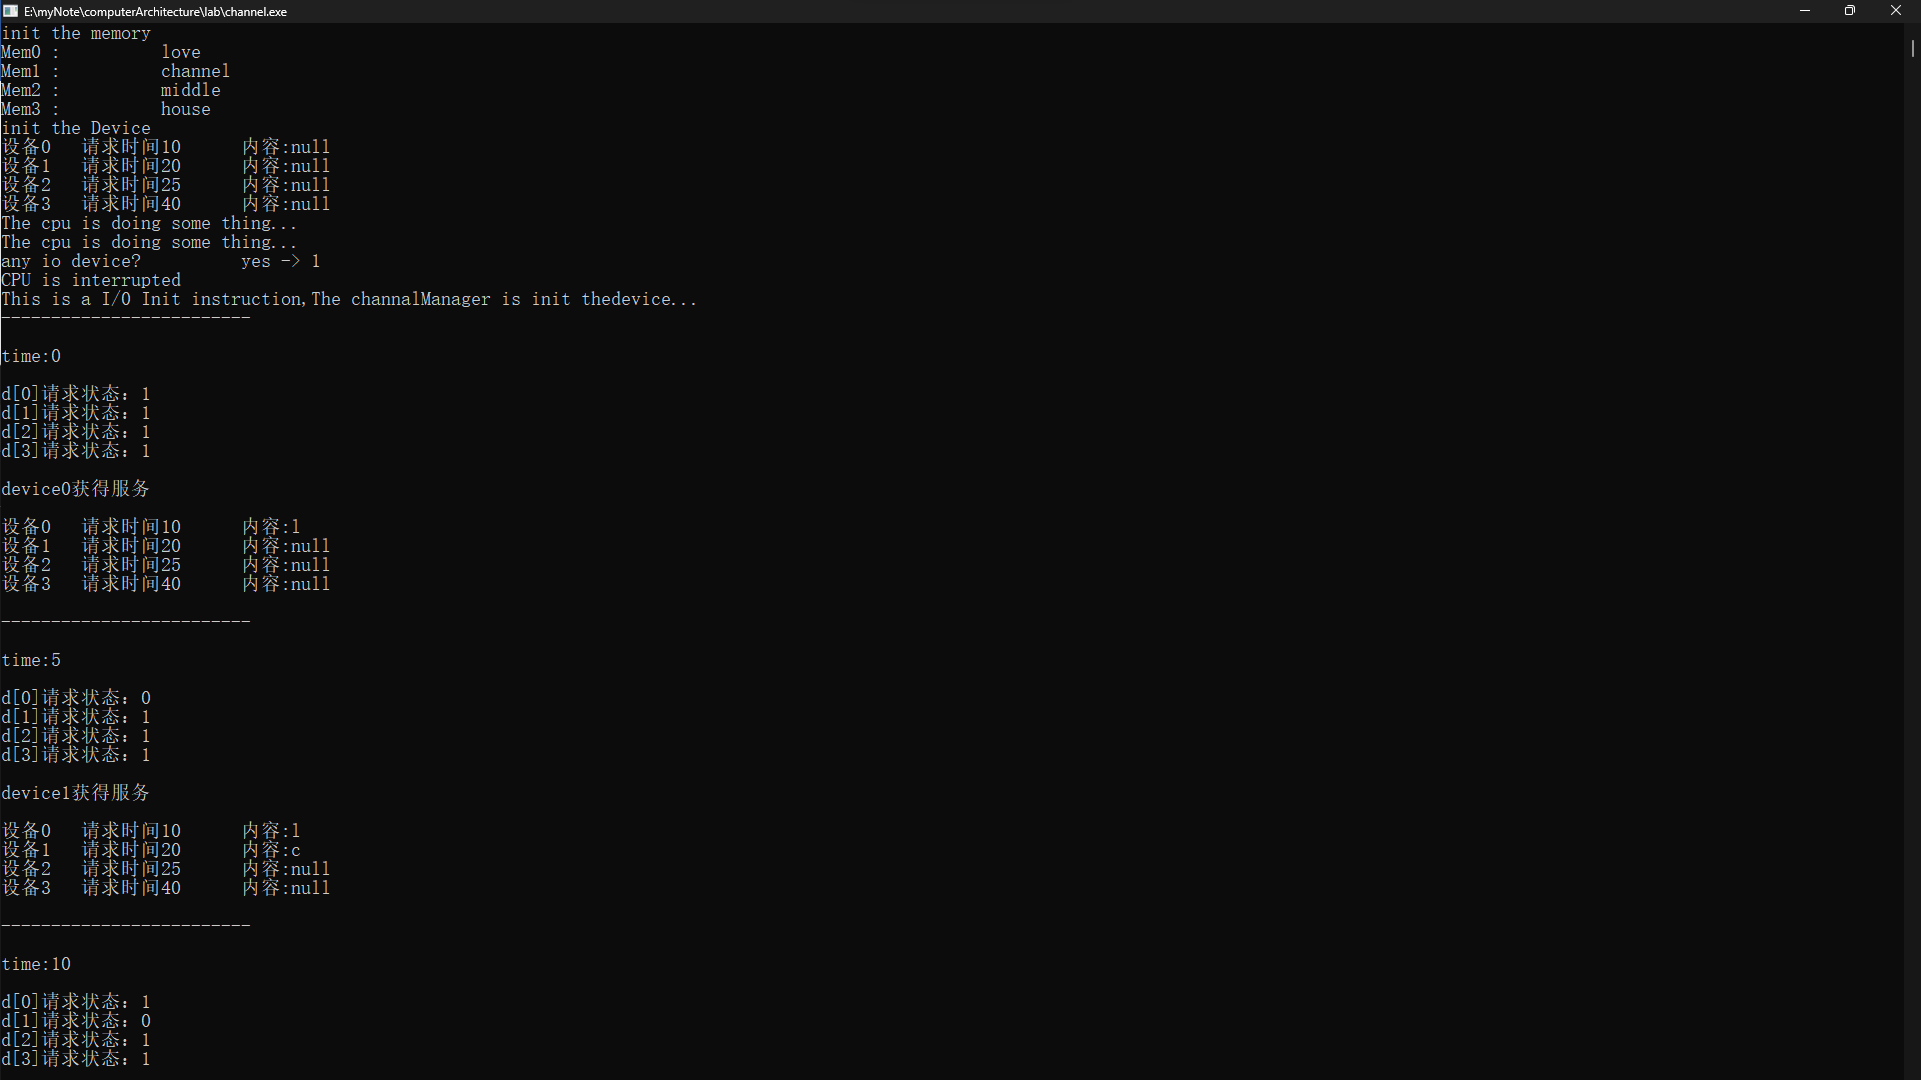
\includegraphics[width=0.7\textwidth]{imgs/7.png}
    \caption{实验三实验结果1}
\end{figure}

\begin{figure}[htbp]
    \centering
    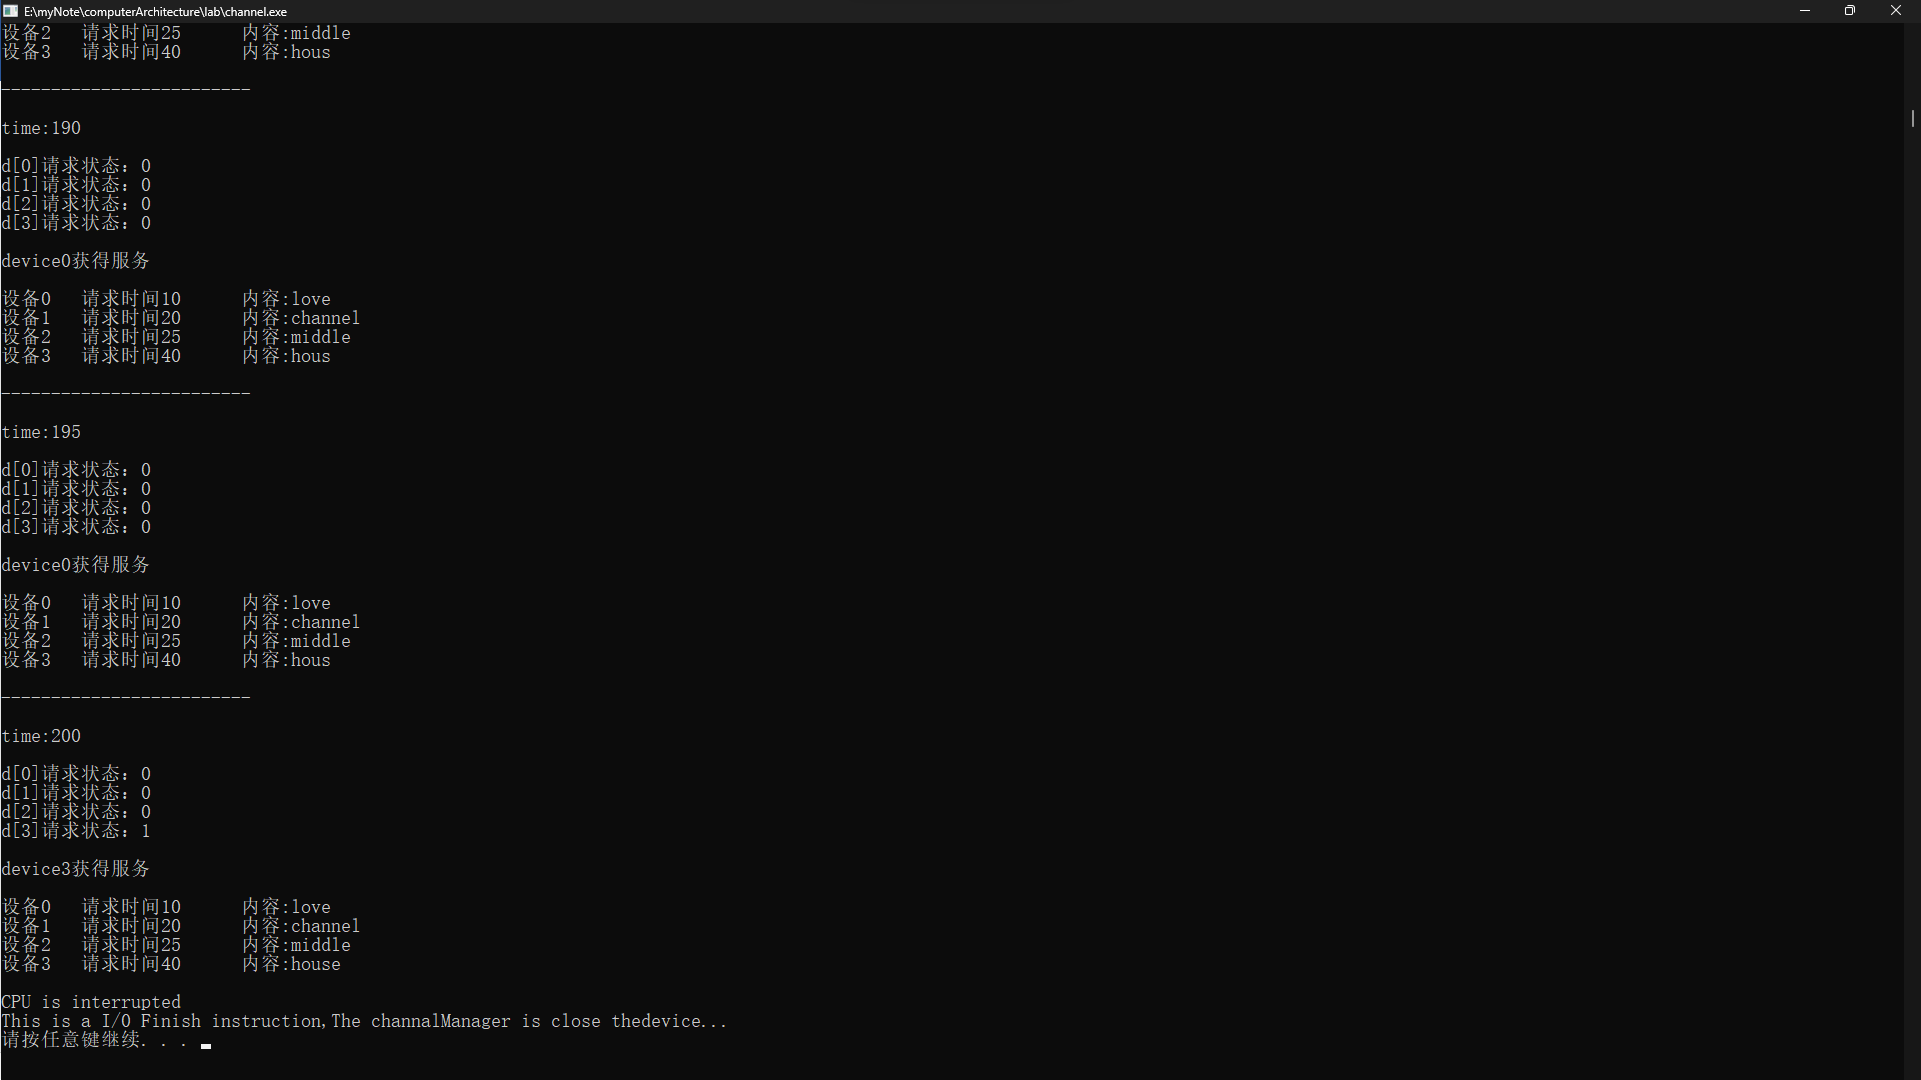
\includegraphics[width=0.7\textwidth]{imgs/8.png}
    \caption{实验三实验结果2}
\end{figure}

\newpage

\section{实验四}
\subsection{实验题目}
单功能流水线调度机构模拟

\subsection{实验目的}
结合数据结构的相关知识,编写流水线调度模拟程序

\subsection{实验内容}
通过模拟单功能流水线调度过程,掌握流水线技术,学会计算流水线的吞吐率、加速比、效率

\begin{enumerate}
    \item 流水线的表示法有三种
    
    连接图、时空图、预约表。对于线性流水线,主要考虑前二种
    \item 流水线的主要特点
    
    在流水线的每一个功能部件的后面都要有一个缓冲器,称为锁存器、闸门寄存器等,它的作用是保存本流水段的执行结果。各流水段的时间应尽量相等,否则回引起阻塞、断流等。
    只有连续提供同类任务才能充分发挥流水线的效率。在流水线的每一个流水线段中都要设置一个流水锁存器。流水线需要有“装入时间”和“排空时间”。只有流水线完全充满时,整个流水线的效率才能得到充分发挥。
\end{enumerate}
\subsection{实验过程}
模拟流水线的过程并不复杂,只需要模拟流水线的每个阶段即可,实验要求的是时空图,因此实现了时空图的算法。

首先定义存储时空图的数据结构,如下:

\begin{lstlisting}[frame=shadowbox] 
    const int SPACE = 4;  // 功能部件数目
    const int NUM = 5;    // 需要流水处理的浮点加指令数目
    const int TIME = NUM + SPACE - 1;  // 存储不同时间段各个功能部件内指令值
    int ts[SPACE][TIME] = {0};  // 初始化时空图
\end{lstlisting}

这里有四个功能部件,分别是:

\begin{itemize}
    \item ED:求阶差 
    \item EA:对阶 
    \item MA:尾数加 
    \item NL:规格化
\end{itemize}

\begin{lstlisting}[frame=shadowbox]
    const string INSTRUCTIONS[] = {"NL", "MA", "EA", "ED"};
\end{lstlisting}

接下来实现时空图的算法,具体实现如下:

\begin{lstlisting}[frame=shadowbox]
    void pipeline(int ts[SPACE][TIME]) {
        int tempSpace = 0;  // 记录处理的指令号
        int tempTime = 0;   // 记录时间轴的变化
        for (int s = SPACE - 1; s >= 0; s--) {
            tempSpace = 1;
            for (int t = tempTime; t < TIME; t++) {
                ts[s][t] = tempSpace++;
            }
            tempTime++;
        }
    }
\end{lstlisting}

\subsection{实验结果}
在这里只放置最后的时空图,完整的时空图可以在程序运行时查看。

\begin{figure}[htbp]
    \centering
    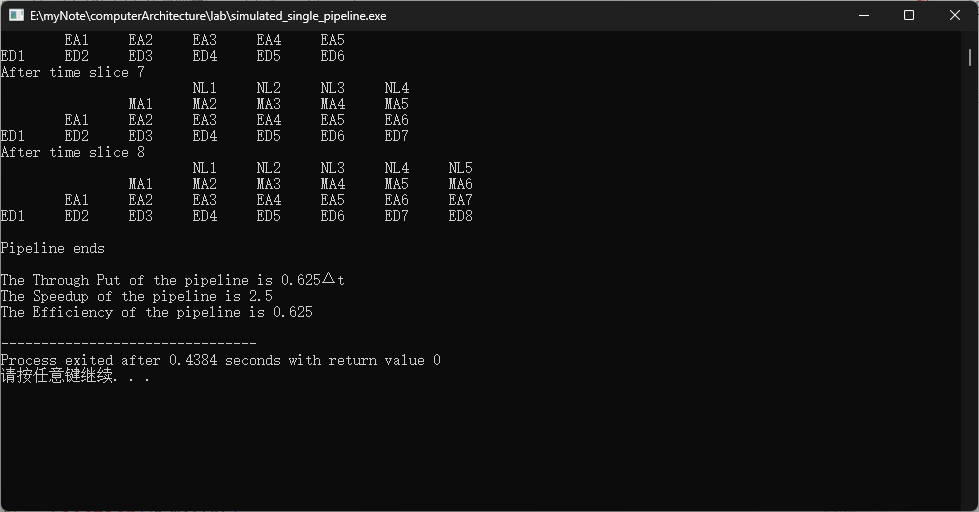
\includegraphics[width=1.0\textwidth]{imgs/9.png}
    \caption{实验四实验结果}
\end{figure}


\newpage

\section{实验总结}

\begin{itemize}
    \item 通过指令操作码霍夫曼编码,我深入理解了指令操作码的编码和解码过程,霍夫曼编码的应用使得指令的表示更为紧凑,减小了存储和传输的开销这个实验提供了对信息理论和编码技术在计算机体系结构中的应用的实际经验
    \item 通过LRU Cache更新算法学到了LRU(最近最少使用)算法,这是一种常用的缓存更新策略。对缓存替换策略的选择有了更深刻的理解,以及对缓存的优化和性能提升有了实际经验。
    \item 通过模拟通道处理过程我对数据在计算机系统中的传输和处理流程有了更深入的理解。理解了通道的工作原理,如何优化数据传输以提高系统性能。
    对并行处理和数据通信有了更为直观的感受。
    \item 通过单功能流水线调度机构模拟学到了流水线调度机构的基本原理,以及如何通过流水线提高指令执行效率。了解了流水线中各个阶段的功能和协同工作的原理    
\end{itemize}

计算机体系结构是一门综合性强、关联度高的课程。通过这门课程,我对计算机硬件和软件之间的交互有了更全面的认识。
编程实验使得理论知识更加具体化,帮助我更好地理解和应用课堂上学到的概念。
实践中遇到的问题和解决方法使我更加熟悉计算机体系结构的实际应用。通过这门课程,我深入了解了计算机系统的各个层次,包括指令级别、流水线、缓存、并行处理等。




\newpage

\section{附录}
\subsection{实验一}
\subsubsection{源代码construct\_huffman\_tree.cpp}
\subsubsection{程序construct\_huffman\_tree.exe}
\subsection{实验二}
\subsubsection{源代码LRU4cache-update.cpp}
\subsubsection{程序LRU4cache-update.exe}
\subsection{实验三}
\subsubsection{源代码class.h \& channel.cpp}
\subsubsection{程序channel.exe}
\subsubsection{完整实验结果}
\begin{lstlisting}[frame=shadowbox]
    init the memory
    Mem0 :          love
    Mem1 :          channel
    Mem2 :          middle
    Mem3 :          house
    init the Device
    设备0   请求时间10      内容:null
    设备1   请求时间20      内容:null
    设备2   请求时间25      内容:null
    设备3   请求时间40      内容:null
    The cpu is doing some thing...
    The cpu is doing some thing...
    any io device?          yes -> 1
    CPU is interrupted
    This is a I/0 Init instruction,The channalManager is init thedevice...
    -------------------------
    
    time:0
    
    d[0]请求状态:1
    d[1]请求状态:1
    d[2]请求状态:1
    d[3]请求状态:1
    
    device0获得服务
    
    设备0   请求时间10      内容:l
    设备1   请求时间20      内容:null
    设备2   请求时间25      内容:null
    设备3   请求时间40      内容:null
    
    -------------------------
    
    time:5
    
    d[0]请求状态:0
    d[1]请求状态:1
    d[2]请求状态:1
    d[3]请求状态:1
    
    device1获得服务
    
    设备0   请求时间10      内容:l
    设备1   请求时间20      内容:c
    设备2   请求时间25      内容:null
    设备3   请求时间40      内容:null
    
    -------------------------
    
    time:10
    
    d[0]请求状态:1
    d[1]请求状态:0
    d[2]请求状态:1
    d[3]请求状态:1
    
    device0获得服务
    
    设备0   请求时间10      内容:lo
    设备1   请求时间20      内容:c
    设备2   请求时间25      内容:null
    设备3   请求时间40      内容:null
    
    -------------------------
    
    time:15
    
    d[0]请求状态:0
    d[1]请求状态:0
    d[2]请求状态:1
    d[3]请求状态:1
    
    device2获得服务
    
    设备0   请求时间10      内容:lo
    设备1   请求时间20      内容:c
    设备2   请求时间25      内容:m
    设备3   请求时间40      内容:null
    
    -------------------------
    
    time:20
    
    d[0]请求状态:1
    d[1]请求状态:1
    d[2]请求状态:0
    d[3]请求状态:1
    
    device0获得服务
    
    设备0   请求时间10      内容:lov
    设备1   请求时间20      内容:c
    设备2   请求时间25      内容:m
    设备3   请求时间40      内容:null
    
    -------------------------
    
    time:25
    
    d[0]请求状态:0
    d[1]请求状态:1
    d[2]请求状态:1
    d[3]请求状态:1
    
    device1获得服务
    
    设备0   请求时间10      内容:lov
    设备1   请求时间20      内容:ch
    设备2   请求时间25      内容:m
    设备3   请求时间40      内容:null
    
    -------------------------
    
    time:30
    
    d[0]请求状态:1
    d[1]请求状态:0
    d[2]请求状态:1
    d[3]请求状态:1
    
    device0获得服务
    
    设备0   请求时间10      内容:love
    设备1   请求时间20      内容:ch
    设备2   请求时间25      内容:m
    设备3   请求时间40      内容:null
    
    -------------------------
    
    time:35
    
    d[0]请求状态:0
    d[1]请求状态:0
    d[2]请求状态:1
    d[3]请求状态:1
    
    device2获得服务
    
    设备0   请求时间10      内容:love
    设备1   请求时间20      内容:ch
    设备2   请求时间25      内容:mi
    设备3   请求时间40      内容:null
    
    -------------------------
    
    time:40
    
    d[0]请求状态:0
    d[1]请求状态:1
    d[2]请求状态:0
    d[3]请求状态:1
    
    device1获得服务
    
    设备0   请求时间10      内容:love
    设备1   请求时间20      内容:cha
    设备2   请求时间25      内容:mi
    设备3   请求时间40      内容:null
    
    -------------------------
    
    time:45
    
    d[0]请求状态:0
    d[1]请求状态:0
    d[2]请求状态:0
    d[3]请求状态:1
    
    device3获得服务
    
    设备0   请求时间10      内容:love
    设备1   请求时间20      内容:cha
    设备2   请求时间25      内容:mi
    设备3   请求时间40      内容:h
    
    -------------------------
    
    time:50
    
    d[0]请求状态:0
    d[1]请求状态:0
    d[2]请求状态:1
    d[3]请求状态:0
    
    device2获得服务
    
    设备0   请求时间10      内容:love
    设备1   请求时间20      内容:cha
    设备2   请求时间25      内容:mid
    设备3   请求时间40      内容:h
    
    -------------------------
    
    time:55
    
    d[0]请求状态:0
    d[1]请求状态:0
    d[2]请求状态:0
    d[3]请求状态:0
    
    device0获得服务
    
    设备0   请求时间10      内容:love
    设备1   请求时间20      内容:cha
    设备2   请求时间25      内容:mid
    设备3   请求时间40      内容:h
    
    -------------------------
    
    time:60
    
    d[0]请求状态:0
    d[1]请求状态:1
    d[2]请求状态:0
    d[3]请求状态:0
    
    device1获得服务
    
    设备0   请求时间10      内容:love
    设备1   请求时间20      内容:chan
    设备2   请求时间25      内容:mid
    设备3   请求时间40      内容:h
    
    -------------------------
    
    time:65
    
    d[0]请求状态:0
    d[1]请求状态:0
    d[2]请求状态:0
    d[3]请求状态:0
    
    device0获得服务
    
    设备0   请求时间10      内容:love
    设备1   请求时间20      内容:chan
    设备2   请求时间25      内容:mid
    设备3   请求时间40      内容:h
    
    -------------------------
    
    time:70
    
    d[0]请求状态:0
    d[1]请求状态:0
    d[2]请求状态:0
    d[3]请求状态:0
    
    device0获得服务
    
    设备0   请求时间10      内容:love
    设备1   请求时间20      内容:chan
    设备2   请求时间25      内容:mid
    设备3   请求时间40      内容:h
    
    -------------------------
    
    time:75
    
    d[0]请求状态:0
    d[1]请求状态:0
    d[2]请求状态:1
    d[3]请求状态:0
    
    device2获得服务
    
    设备0   请求时间10      内容:love
    设备1   请求时间20      内容:chan
    设备2   请求时间25      内容:midd
    设备3   请求时间40      内容:h
    
    -------------------------
    
    time:80
    
    d[0]请求状态:0
    d[1]请求状态:1
    d[2]请求状态:0
    d[3]请求状态:1
    
    device1获得服务
    
    设备0   请求时间10      内容:love
    设备1   请求时间20      内容:chann
    设备2   请求时间25      内容:midd
    设备3   请求时间40      内容:h
    
    -------------------------
    
    time:85
    
    d[0]请求状态:0
    d[1]请求状态:0
    d[2]请求状态:0
    d[3]请求状态:1
    
    device3获得服务
    
    设备0   请求时间10      内容:love
    设备1   请求时间20      内容:chann
    设备2   请求时间25      内容:midd
    设备3   请求时间40      内容:ho
    
    -------------------------
    
    time:90
    
    d[0]请求状态:0
    d[1]请求状态:0
    d[2]请求状态:0
    d[3]请求状态:0
    
    device0获得服务
    
    设备0   请求时间10      内容:love
    设备1   请求时间20      内容:chann
    设备2   请求时间25      内容:midd
    设备3   请求时间40      内容:ho
    
    -------------------------
    
    time:95
    
    d[0]请求状态:0
    d[1]请求状态:0
    d[2]请求状态:0
    d[3]请求状态:0
    
    device0获得服务
    
    设备0   请求时间10      内容:love
    设备1   请求时间20      内容:chann
    设备2   请求时间25      内容:midd
    设备3   请求时间40      内容:ho
    
    -------------------------
    
    time:100
    
    d[0]请求状态:0
    d[1]请求状态:1
    d[2]请求状态:1
    d[3]请求状态:0
    
    device1获得服务
    
    设备0   请求时间10      内容:love
    设备1   请求时间20      内容:channe
    设备2   请求时间25      内容:midd
    设备3   请求时间40      内容:ho
    
    -------------------------
    
    time:105
    
    d[0]请求状态:0
    d[1]请求状态:0
    d[2]请求状态:1
    d[3]请求状态:0
    
    device2获得服务
    
    设备0   请求时间10      内容:love
    设备1   请求时间20      内容:channe
    设备2   请求时间25      内容:middl
    设备3   请求时间40      内容:ho
    
    -------------------------
    
    time:110
    
    d[0]请求状态:0
    d[1]请求状态:0
    d[2]请求状态:0
    d[3]请求状态:0
    
    device0获得服务
    
    设备0   请求时间10      内容:love
    设备1   请求时间20      内容:channe
    设备2   请求时间25      内容:middl
    设备3   请求时间40      内容:ho
    
    -------------------------
    
    time:115
    
    d[0]请求状态:0
    d[1]请求状态:0
    d[2]请求状态:0
    d[3]请求状态:0
    
    device0获得服务
    
    设备0   请求时间10      内容:love
    设备1   请求时间20      内容:channe
    设备2   请求时间25      内容:middl
    设备3   请求时间40      内容:ho
    
    -------------------------
    
    time:120
    
    d[0]请求状态:0
    d[1]请求状态:1
    d[2]请求状态:0
    d[3]请求状态:1
    
    device1获得服务
    
    设备0   请求时间10      内容:love
    设备1   请求时间20      内容:channel
    设备2   请求时间25      内容:middl
    设备3   请求时间40      内容:ho
    
    -------------------------
    
    time:125
    
    d[0]请求状态:0
    d[1]请求状态:0
    d[2]请求状态:1
    d[3]请求状态:1
    
    device2获得服务
    
    设备0   请求时间10      内容:love
    设备1   请求时间20      内容:channel
    设备2   请求时间25      内容:middle
    设备3   请求时间40      内容:ho
    
    -------------------------
    
    time:130
    
    d[0]请求状态:0
    d[1]请求状态:0
    d[2]请求状态:0
    d[3]请求状态:1
    
    device3获得服务
    
    设备0   请求时间10      内容:love
    设备1   请求时间20      内容:channel
    设备2   请求时间25      内容:middle
    设备3   请求时间40      内容:hou
    
    -------------------------
    
    time:135
    
    d[0]请求状态:0
    d[1]请求状态:0
    d[2]请求状态:0
    d[3]请求状态:0
    
    device0获得服务
    
    设备0   请求时间10      内容:love
    设备1   请求时间20      内容:channel
    设备2   请求时间25      内容:middle
    设备3   请求时间40      内容:hou
    
    -------------------------
    
    time:140
    
    d[0]请求状态:0
    d[1]请求状态:0
    d[2]请求状态:0
    d[3]请求状态:0
    
    device0获得服务
    
    设备0   请求时间10      内容:love
    设备1   请求时间20      内容:channel
    设备2   请求时间25      内容:middle
    设备3   请求时间40      内容:hou
    
    -------------------------
    
    time:145
    
    d[0]请求状态:0
    d[1]请求状态:0
    d[2]请求状态:0
    d[3]请求状态:0
    
    device0获得服务
    
    设备0   请求时间10      内容:love
    设备1   请求时间20      内容:channel
    设备2   请求时间25      内容:middle
    设备3   请求时间40      内容:hou
    
    -------------------------
    
    time:150
    
    d[0]请求状态:0
    d[1]请求状态:0
    d[2]请求状态:0
    d[3]请求状态:0
    
    device0获得服务
    
    设备0   请求时间10      内容:love
    设备1   请求时间20      内容:channel
    设备2   请求时间25      内容:middle
    设备3   请求时间40      内容:hou
    
    -------------------------
    
    time:155
    
    d[0]请求状态:0
    d[1]请求状态:0
    d[2]请求状态:0
    d[3]请求状态:0
    
    device0获得服务
    
    设备0   请求时间10      内容:love
    设备1   请求时间20      内容:channel
    设备2   请求时间25      内容:middle
    设备3   请求时间40      内容:hou
    
    -------------------------
    
    time:160
    
    d[0]请求状态:0
    d[1]请求状态:0
    d[2]请求状态:0
    d[3]请求状态:1
    
    device3获得服务
    
    设备0   请求时间10      内容:love
    设备1   请求时间20      内容:channel
    设备2   请求时间25      内容:middle
    设备3   请求时间40      内容:hous
    
    -------------------------
    
    time:165
    
    d[0]请求状态:0
    d[1]请求状态:0
    d[2]请求状态:0
    d[3]请求状态:0
    
    device0获得服务
    
    设备0   请求时间10      内容:love
    设备1   请求时间20      内容:channel
    设备2   请求时间25      内容:middle
    设备3   请求时间40      内容:hous
    
    -------------------------
    
    time:170
    
    d[0]请求状态:0
    d[1]请求状态:0
    d[2]请求状态:0
    d[3]请求状态:0
    
    device0获得服务
    
    设备0   请求时间10      内容:love
    设备1   请求时间20      内容:channel
    设备2   请求时间25      内容:middle
    设备3   请求时间40      内容:hous
    
    -------------------------
    
    time:175
    
    d[0]请求状态:0
    d[1]请求状态:0
    d[2]请求状态:0
    d[3]请求状态:0
    
    device0获得服务
    
    设备0   请求时间10      内容:love
    设备1   请求时间20      内容:channel
    设备2   请求时间25      内容:middle
    设备3   请求时间40      内容:hous
    
    -------------------------
    
    time:180
    
    d[0]请求状态:0
    d[1]请求状态:0
    d[2]请求状态:0
    d[3]请求状态:0
    
    device0获得服务
    
    设备0   请求时间10      内容:love
    设备1   请求时间20      内容:channel
    设备2   请求时间25      内容:middle
    设备3   请求时间40      内容:hous
    
    -------------------------
    
    time:185
    
    d[0]请求状态:0
    d[1]请求状态:0
    d[2]请求状态:0
    d[3]请求状态:0
    
    device0获得服务
    
    设备0   请求时间10      内容:love
    设备1   请求时间20      内容:channel
    设备2   请求时间25      内容:middle
    设备3   请求时间40      内容:hous
    
    -------------------------
    
    time:190
    
    d[0]请求状态:0
    d[1]请求状态:0
    d[2]请求状态:0
    d[3]请求状态:0
    
    device0获得服务
    
    设备0   请求时间10      内容:love
    设备1   请求时间20      内容:channel
    设备2   请求时间25      内容:middle
    设备3   请求时间40      内容:hous
    
    -------------------------
    
    time:195
    
    d[0]请求状态:0
    d[1]请求状态:0
    d[2]请求状态:0
    d[3]请求状态:0
    
    device0获得服务
    
    设备0   请求时间10      内容:love
    设备1   请求时间20      内容:channel
    设备2   请求时间25      内容:middle
    设备3   请求时间40      内容:hous
    
    -------------------------
    
    time:200
    
    d[0]请求状态:0
    d[1]请求状态:0
    d[2]请求状态:0
    d[3]请求状态:1
    
    device3获得服务
    
    设备0   请求时间10      内容:love
    设备1   请求时间20      内容:channel
    设备2   请求时间25      内容:middle
    设备3   请求时间40      内容:house
    
    CPU is interrupted
    This is a I/0 Finish instruction,The channalManager is close thedevice...
\end{lstlisting}
\subsection{实验四}
\subsubsection{源代码simulated\_single\_pipeline.cpp}
\subsubsection{程序simulated\_single\_pipeline.exe}
\subsubsection{完整实验结果}
\begin{lstlisting}[frame=shadowbox]
Pipeline begins

After time slice 1



ED1
After time slice 2


        EA1
ED1     ED2
After time slice 3

                MA1
        EA1     EA2
ED1     ED2     ED3
After time slice 4
                        NL1
                MA1     MA2
        EA1     EA2     EA3
ED1     ED2     ED3     ED4
After time slice 5
                        NL1     NL2
                MA1     MA2     MA3
        EA1     EA2     EA3     EA4
ED1     ED2     ED3     ED4     ED5
After time slice 6
                        NL1     NL2     NL3
                MA1     MA2     MA3     MA4
        EA1     EA2     EA3     EA4     EA5
ED1     ED2     ED3     ED4     ED5     ED6
After time slice 7
                        NL1     NL2     NL3     NL4
                MA1     MA2     MA3     MA4     MA5
        EA1     EA2     EA3     EA4     EA5     EA6
ED1     ED2     ED3     ED4     ED5     ED6     ED7
After time slice 8
                        NL1     NL2     NL3     NL4     NL5
                MA1     MA2     MA3     MA4     MA5     MA6
        EA1     EA2     EA3     EA4     EA5     EA6     EA7
ED1     ED2     ED3     ED4     ED5     ED6     ED7     ED8

Pipeline ends

The Through Put of the pipeline is 0.625Δt
The Speedup of the pipeline is 2.5
The Efficiency of the pipeline is 0.625

\end{lstlisting}





\end{document}
